%! Licence = CC BY-NC-SA 4.0

%! Author = gianfluetsch, mariuszindel
%! Date = 30. Dez 2021
%! Project = cydef_summary


\section{Mail Security}
DKIM, SPF und DMARC sind Standards, die verschiedene Aspekte der E-Mail-Authentifizierung ermöglichen.
\begin{center}
    \vspace{-8pt}
    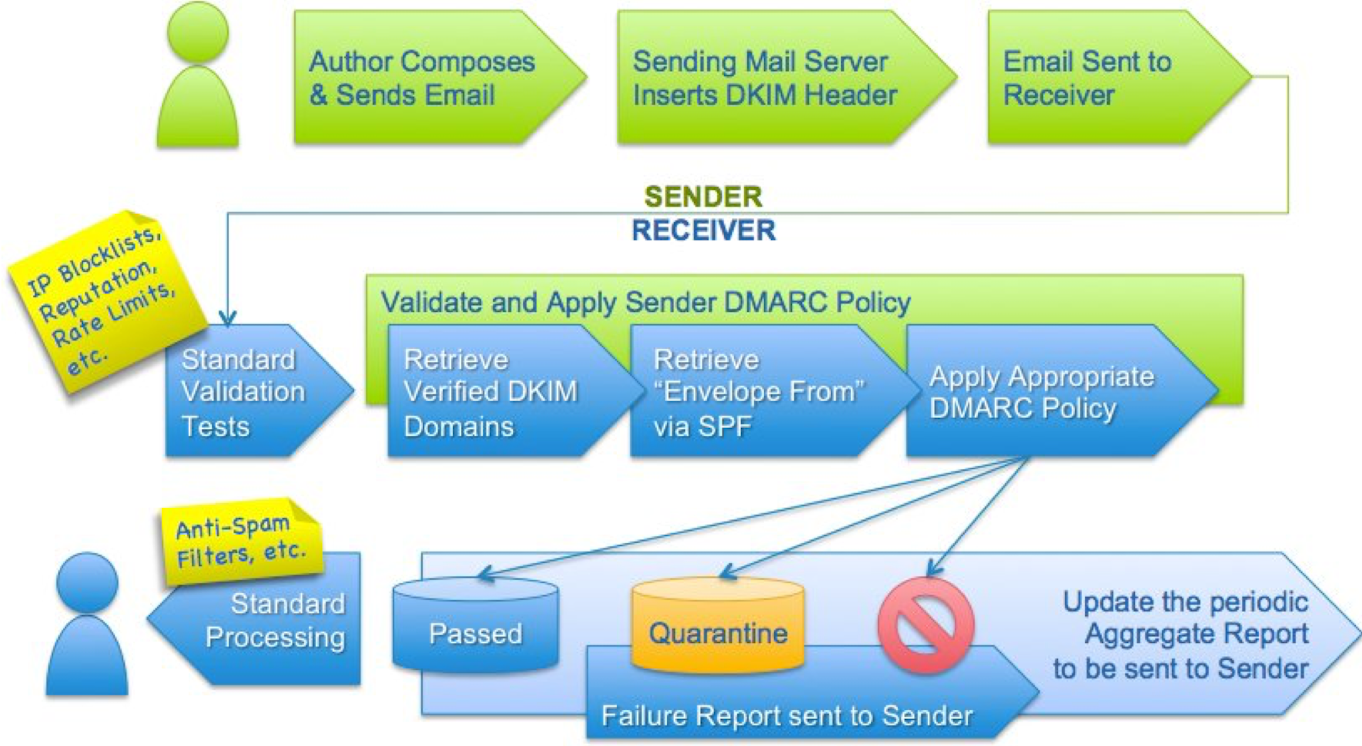
\includegraphics[width=.8\linewidth]{./img/07-mail_security/overview}
    \vspace{-8pt}
\end{center}
\begin{center}
    \vspace{-8pt}
    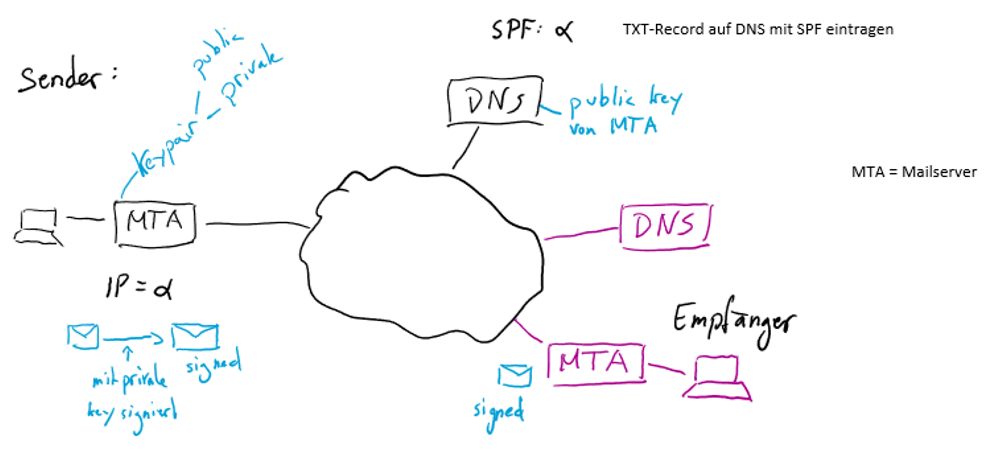
\includegraphics[width=1.0\linewidth]{./img/07-mail_security/spf_overview}
    \vspace{-8pt}
\end{center}

\subsection{SPF: Sender Policy Framework}
Mit \textit{SPF} können Absender festlegen, welche IP-Adressen E-Mails für eine bestimmte Domäne senden dürfen.
DNS TXT-Entry mit allen IP-Ranges, von welchen ein Mail mit dieser Domain verschickt werden darf.
Alles was nicht von den outgoing Mail/MX Servern stammt, ist ''Fake''und wird in Spam verschoben oder gar nicht erst zugestellt.\\

\textit{SPF} ist besonders effizient gegen \textcolor{red}{\textbf{Phishing-Angriffe}}.

\subsubsection{Ablauf}
Auf dem \textbf{DNS} kann eingegrenzt werden, wer (welche IP) alles ein Mail verschicken darf.
\begin{itemize}
    \item \textcolor{purple}{\textbf{MTA}} macht \textbf{DNS-Lookup} und fragt diesen an, welche IPs berechtig sind Mails zu versenden.
    \begin{itemize}
        \item IP-$\alpha$ (TCP) $\rightarrow$ DNS-Lookup $\rightarrow$ SPF@ost.ch
        \item Falls $\alpha$ darin enthalten $\rightarrow$ ok
    \end{itemize}
\end{itemize}

Wenn Empfänger SPF-Policy nicht enforced, ist egal was der Sender konfiguriert hat. Empfänger-MTA interessiert das nicht.\\

\subsubsection{Header}
Wenn SPF verwendet wird, sollte dies im Header/ Log ersichtlich sein!
\begin{center}
    \vspace{-8pt}
    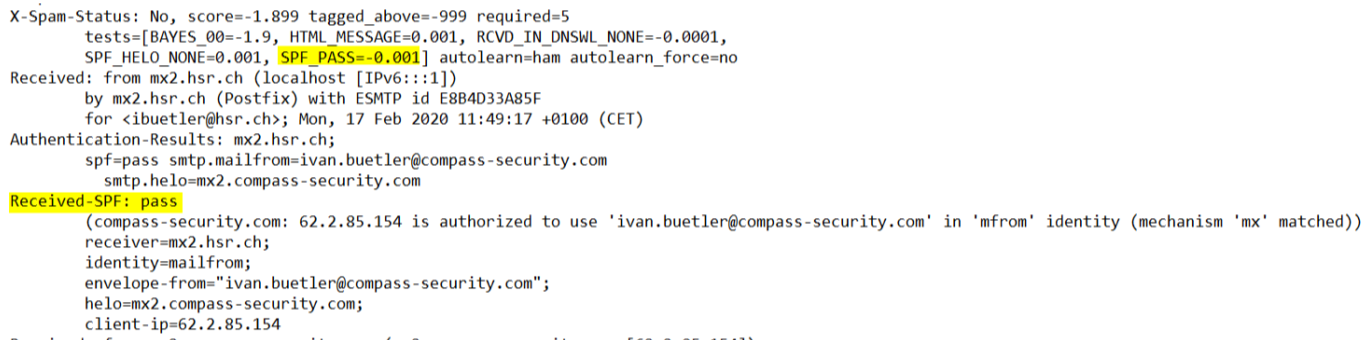
\includegraphics[width=1.0\linewidth]{./img/07-mail_security/spf}
    \vspace{-8pt}
\end{center}
\begin{center}
    \vspace{-8pt}
    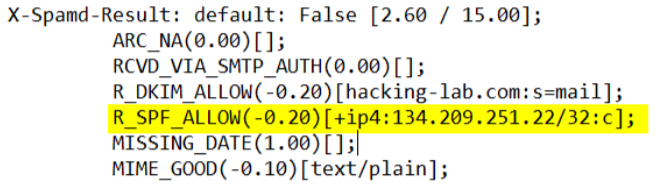
\includegraphics[width=.6\linewidth]{./img/07-mail_security/spf2}
    \vspace{-8pt}
\end{center}
\begin{center}
    \vspace{-8pt}
    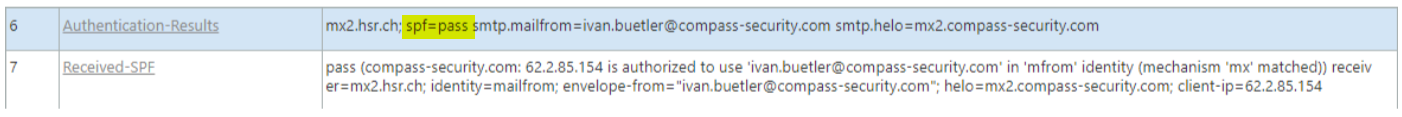
\includegraphics[width=1.0\linewidth]{./img/07-mail_security/spf3}
    \vspace{-8pt}
\end{center}

\subsection{DKIM: DomainKeys Identified Mail}
\textcolor{cyan}{\textbf{DKIM}} stellt einen Encryption Key und eine digitale Signatur bereit, die nachweisen, dass eine E-Mail-Nachricht nicht gefälscht oder verändert wurde.
DKIM fügt dazu dem E-Mail Header eine digitale Signatur hinzu, welche vom Empfänger mit dem \textit{Public Key} (welcher auf dem DNS Server gespeichert ist) validiert werden kann.\\

Der Mail-Server hat ein Public/Private Key Cert Pair. Der Public Key wird via weltweit verfügbaren DNS veröffentlicht. 
Der Plaintext in einem Mail wird gehasht und im Header gespeichert. 
Der Header wird wieder mit dem Private Key signiert (also inkl. dem Hash des Plain Texts). 
Empfänger Mail-Server kann nun mit dem öffentlich verfügbaren Public Key feststellen, ob der Sender der ist der er angibt (Korrekte Firma mit Zugriff auf Private/Public Pair). 
Durch das Signieren ist auch klar, dass der Content ''in Transit'' nicht verändert wurde.\\

\textit{DKIM} ist besonders effizient gegen \textcolor{red}{\textbf{Man-in-the-middle-Angriffen}}.

\subsubsection{Ablauf}
\begin{itemize}
    \item Mailserver signiert Mail mit private Key
    \item Mail kommt beim  \textcolor{purple}{MTA} an und dieser prüft ob Mail signiert ist
    \begin{itemize}
        \item Wenn Signatur vorhanden $\rightarrow$ \textbf{DNS-lookup} für public key $\rightarrow$ prüft Signatur von Mail mit dem public key des \textbf{DNS Servers}\\
    \end{itemize}
\end{itemize}

\subsubsection{Header}
Wenn DKIM verwendet wird, sollte dies im Header/ Log ersichtlich sein!
\begin{center}
    \vspace{-8pt}
    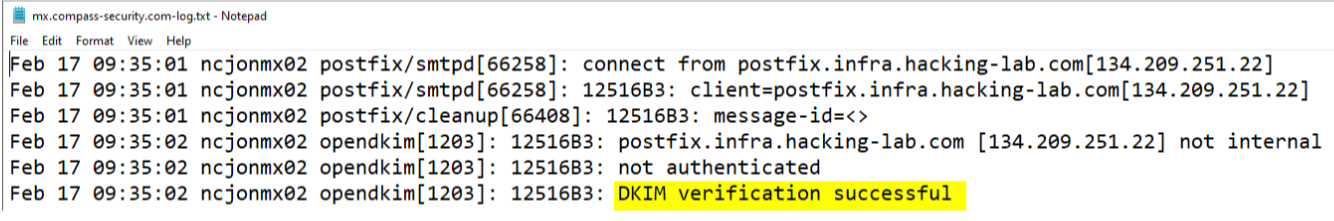
\includegraphics[width=1.0\linewidth]{./img/07-mail_security/dkim}
    \vspace{-8pt}
\end{center}
Due to the MX of Compass, the \textit{DKIM} service is initialized. But the headers from the OWA do not have DKIM headers applied. Thus, DKIM isn't used!
\begin{center}
    \vspace{-8pt}
    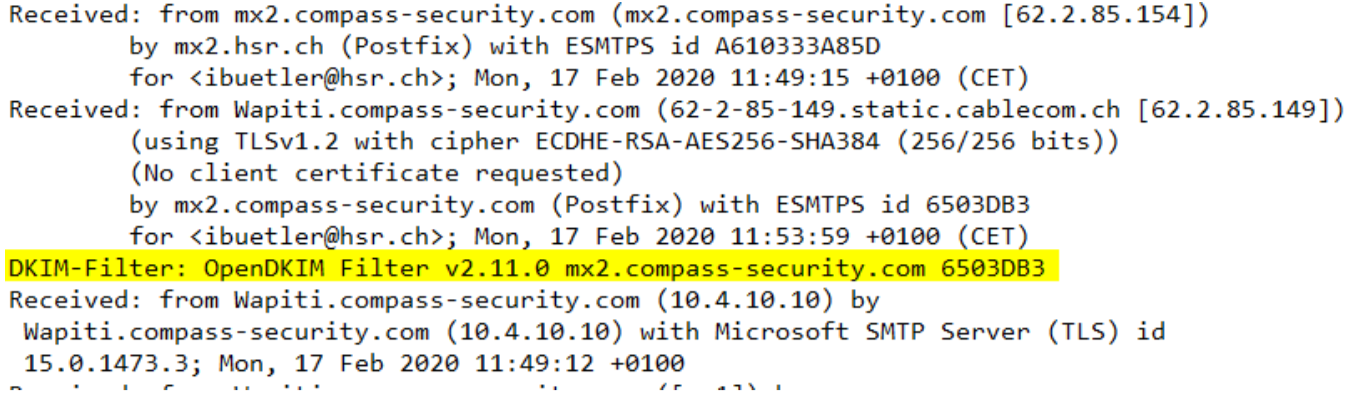
\includegraphics[width=.8\linewidth]{./img/07-mail_security/dkim2}
    \vspace{-8pt}
\end{center}

\columnbreak

\subsection{DMARC: (Domain-based Message Authentication, Reporting, and Conformance}
\textit{DMARC} prüft, ob die SPF sowie DKIM Checks erfüllt werden. Nun können Regeln definiert werden, die bei nicht-bestehen der Checks angewendet werden. Das kann z.B. das rejecten des Mails, in Quarantäne stellen oder das Verschieben in den Spamordner sein.
Policies werden im DNS als TXT-Einträge veröffentlicht und geben an, was ein E-Mail-Empfänger mit E-Mails mit nicht-bestandenen Checks tun soll, die er erhält.\\

DMARC sind TXT DNS-Entries die definieren, was der Empfänger mit Mails von seiner Domain(DNS Entry Domain) machen soll. 
Wo er Spam oder Malware in den Mails dem Absender melden soll (Contact-to-Adresse). 
Vorallem aber relevant, wenn Mail-Header verändert werden (sending in name of someone else) und so der effektive Eigentümer benachrichtigt werden kann, dass ein Fraud passiert ist.

\subsubsection{Header}
\textbf{DMARC is available!}
\begin{center}
    \vspace{-8pt}
    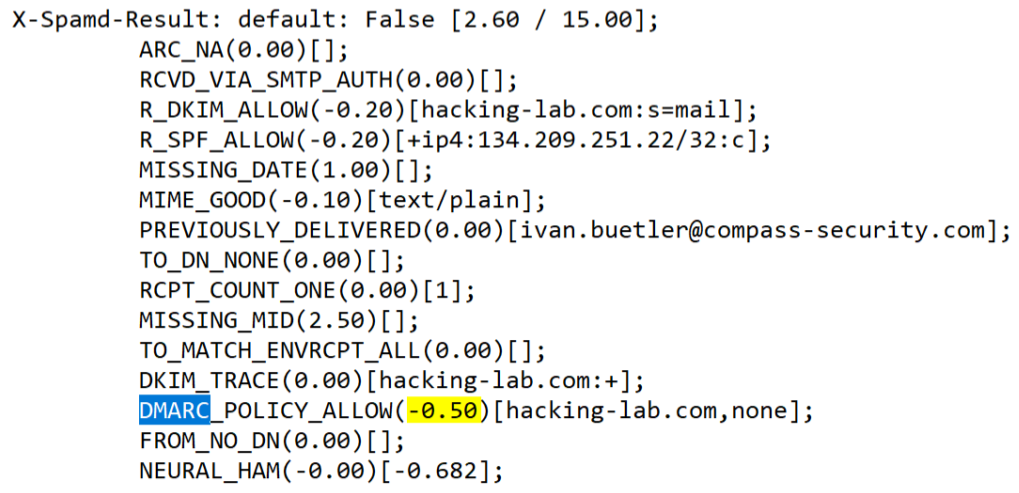
\includegraphics[width=1.0\linewidth]{./img/07-mail_security/dmarc}
    \vspace{-8pt}
\end{center}
\textbf{DMARC not available (NA)!}
\begin{center}
    \vspace{-8pt}
    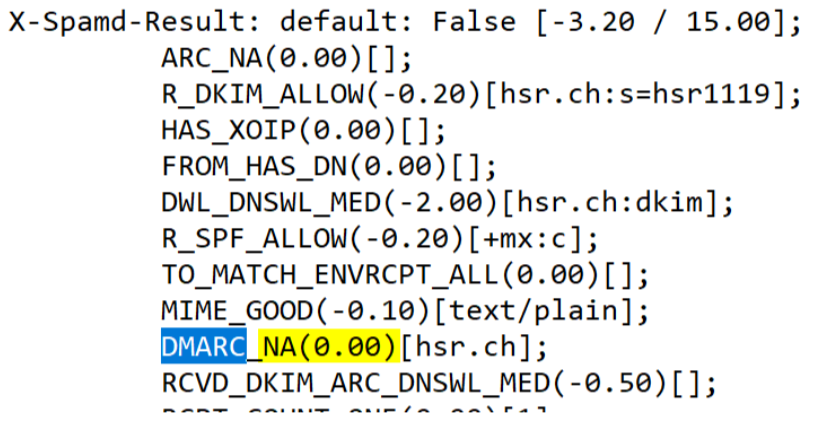
\includegraphics[width=1.0\linewidth]{./img/07-mail_security/dmarc2}
    \vspace{-8pt}
\end{center}


\subsection{Opportunistic TLS Encryption}
By checking the pcap files, one can see the \textit{STARTTLS} messages which will let us know tls encryption has been used.

\begin{center}
   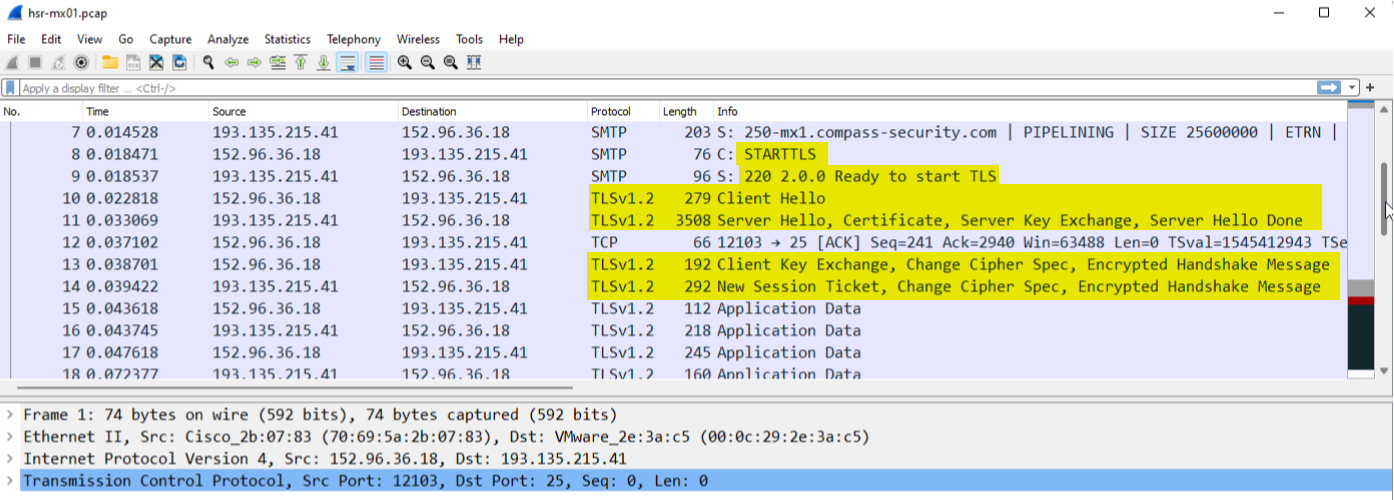
\includegraphics[width=1.0\linewidth]{./img/07-mail_security/tls_encryption}
\end{center}


\subsection{Spam Mails}
\subsubsection{Tools}
\begin{itemize}
    \item DNSTwister
\end{itemize}



